\documentclass{beamer}
\usepackage[utf8]{inputenc}
\usepackage[inline]{enumitem}
\usepackage{pdfpages}
\usepackage{listings}
\usepackage{subcaption}
\usepackage{wasysym}
\usepackage[export]{adjustbox}[2011/08/13]
\usetheme{cern}

\newcommand{\btVFill}{\vskip0pt plus 1filll}

% fix tilde
% \newcommand{\propertilde}{\raise.17ex\hbox{$\scriptstyle\mathtt{\sim}$}}

% \setbeameroption{show notes on second screen=right}

%The CERN logo is legally protected. Please visit http://cern.ch/copyright for
%information on the terms of use of CERN content, including the CERN logo.

% The optional `\author` command defines the author and is displayed in the
%slide produced by the `\titlepage` command.
\author{Corne Lukken}

% The optional `\title` command defines the title and is displayed in the slide
%produced by the `\titlepage` command.
\title{OpenCL Fast Fourier Transform}

% The optional `\subtitle` command will add a smaller title below the main one,
%and will not be displayed in any of the slides' footer.
\subtitle{Real-time$^*$ GPGPU}

% The optional `\date` command will display a custom free text date on the all
%of the slides' footer. If omitted today's date will be used.
%\date{Monday, 1st January 2018}

% ------------------------------------------------------------------------%
% Proper Python Syntax Highlighting                                       %
% Author: redmode
% https://tex.stackexchange.com/questions/83882/how-to-highlight-python   %
% -syntax-in-latex-listings-lstinputlistings-command#83883                %
% ----------------------------------------------------------------------- %

% Default fixed font does not support bold face
\DeclareFixedFont{\ttb}{T1}{txtt}{bx}{n}{6} % for bold
\DeclareFixedFont{\ttm}{T1}{txtt}{m}{n}{6}  % for normal

% Custom colors
\definecolor{deepblue}{rgb}{0,0,0.5}
\definecolor{deepred}{rgb}{0.6,0,0}
\definecolor{deepgreen}{rgb}{0,0.5,0}

% Python style for highlighting
\newcommand\pythonstyle{
	\lstset{
		language=Python,
		basicstyle=\ttm,
		showstringspaces=false,
		tabsize=2,
		aboveskip=0.1cm,
		belowskip=0.1cm,
		otherkeywords={self},             % Add keywords here
		keywordstyle=\ttb\color{deepblue},
		emph={MyClass,__init__},          % Custom highlighting
		emphstyle=\ttb\color{deepred},    % Custom highlighting style
		stringstyle=\color{deepgreen},
		frame=tb,                          % Any extra options here
		prebreak=\textbackslash,
		linewidth=7.00cm,
		breaklines=true,
	}
}

% Python environment
\lstnewenvironment{python}[1][] {
	\pythonstyle\lstset{#1}
}{}

% Python for inline
\newcommand\pythoninline[1]{{\pythonstyle\lstinline!#1!}}

% Python for external file
\newcommand\pythonexternal[2][]{{\pythonstyle\lstinputlisting[#1]{#2}}}

\newcommand\pythonfullstyle{
	\lstset{
		language=Python,
		basicstyle=\ttm,
		showstringspaces=false,
		tabsize=2,
		aboveskip=0.1cm,
		belowskip=0.1cm,
		otherkeywords={self},             % Add keywords here
		keywordstyle=\ttb\color{deepblue},
		emph={MyClass,__init__},          % Custom highlighting
		emphstyle=\ttb\color{deepred},    % Custom highlighting style
		stringstyle=\color{deepgreen},
		frame=tb,                          % Any extra options here
		prebreak=\textbackslash,
		linewidth=11.00cm,
		breaklines=true,
	}
}

% Python environment
\lstnewenvironment{pythonfull}[1][] {
	\pythonfullstyle\lstset{#1}
}{}

% Python for inline
\newcommand\pythonfullinline[1]{{\pythonfullstyle\lstinline!#1!}}

% Python for external file
\newcommand\pythonfullexternal[2][]{{\pythonfullstyle\lstinputlisting[#1]{#2}}}

% ----------------------------------------------------------------------- %

% Bash style for highlighting
\newcommand\bashstyle{
	\lstset{
		language=Bash,
		basicstyle=\ttm,
		showstringspaces=false,
		tabsize=2,
		%commentstyle=itshape,
		aboveskip=0.1cm,
		belowskip=0.1cm,
		prebreak=\textbackslash,
		extendedchars=true,
		mathescape=false,
		% literate= {\$}{{\textcolor{blue}{\$}}}1 {&}{{\textcolor{blue}{\&}}}1 {/n}{{\textcolor{green}{\textbackslash n}}}1,
		linewidth=11cm,
		breaklines=true
	}
}

% Bash environment
\lstnewenvironment{bash}[1][] {
	\bashstyle\lstset{#1}
}{}

% Bash for inline
\newcommand\bashinline[1]{{\bashstyle\lstinline!#1!}}

% Bash for external file
\newcommand\bashexternal[2][]{{\bashstyle\lstinputlisting[#1]{#2}}}


\begin{document}

% \frontcover

% The optional `\titlepage` command will create a slide with the presentation's
%title, subtitle and author.
\frame{\titlepage}

% The optional `\tableofcontents` command will automatically create a table of
%contents based pm the sections.
% \frame{\tableofcontents}

% \section{Introduction}

\begin{frame}{Discrete Fourier Transform}
	\begingroup
	\small
	\begin{columns}
		\begin{column}{0.45\textwidth}
			\textit{Conversion from time domain to frequency domain.}
			\begin{itemize}
				\item{Uses complex numbers}
				\item{Rotates input around center of complex plane}
				\item{Strength at a frequency is magnitude from center.}
				\item{Is linear and has an inverse}
				\item{Complexity $\mathcal{O}(n^3)$}
			\end{itemize}
		\end{column}
		\begin{column}{0.55\textwidth}
			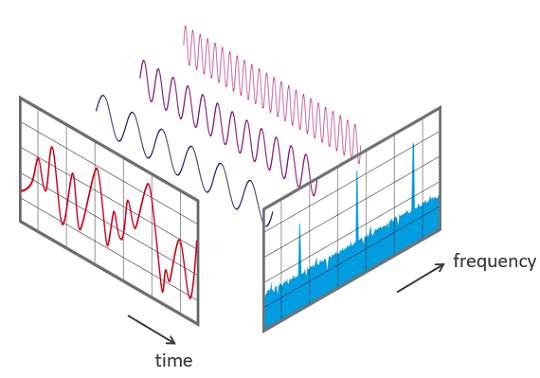
\includegraphics[width=0.7\textwidth,center]{resources/images/fft.png}
			\begin{figure}
				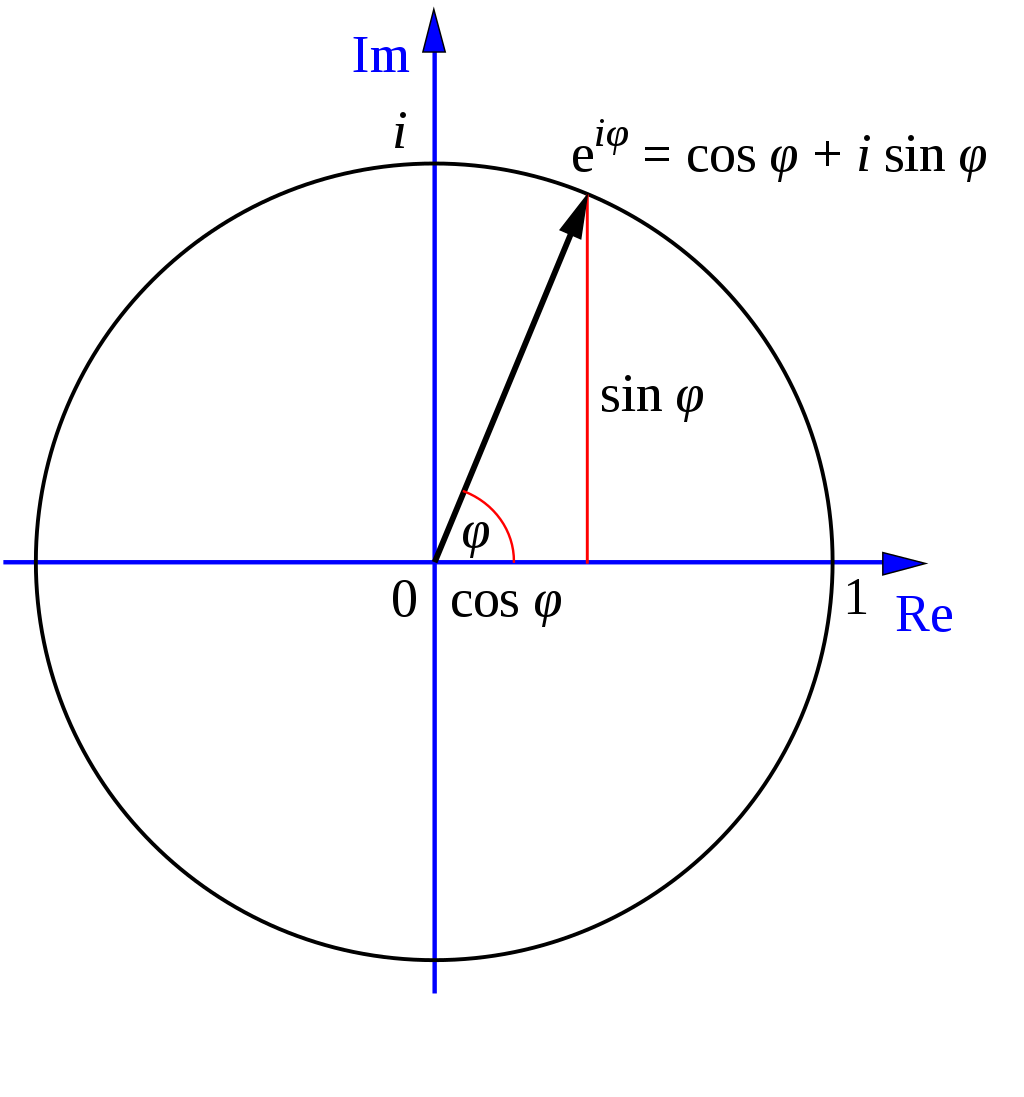
\includegraphics[width=0.45\textwidth,center]{resources/images/euler.png}
				\caption{\tiny Image from Gunther CC-BY-SA 3.0}
			\end{figure}
		\end{column}
	\end{columns}
	\endgroup
\end{frame}

\begin{frame}{Cooley-Tukey Fast Fourier Transform}
	\begingroup
	\small
	\begin{columns}
		\begin{column}{0.45\textwidth}
			\begin{itemize}
				\item Divide and conquer, split in two recursively
				\item Input needs to be power of two
				\item Merge with butterfly operation
				\item Complexity $\mathcal{O}(n\log{}n)$
			\end{itemize}
		\end{column}
		\begin{column}{0.55\textwidth}
			\begin{figure}
				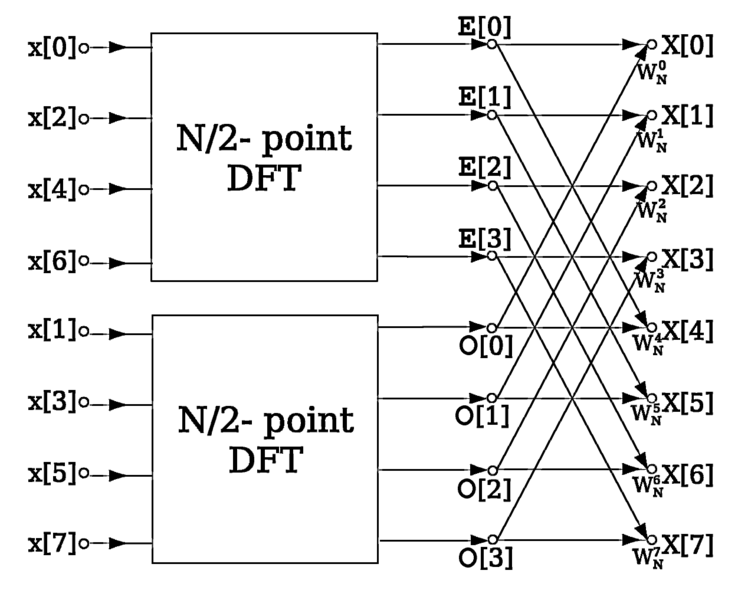
\includegraphics[width=0.7\textwidth,center]{resources/images/tukey.png}
				\caption{\tiny Image from Virens CC-BY 3.0}
			\end{figure}
		\end{column}
	\end{columns}
	\endgroup
\end{frame}

\begin{frame}{The goal}
	\begingroup
	\small
	Compute (Nuttall) Windowing, FFT and magnitudes within 16.66ms using
	OpenCL.
	\begin{itemize}
		\item Timing requirement includes memory transfers
		\item When goal is reached increase \textit{bin} size
		\item Windowing required to prevent spectrum leakage
		(incorrect results).
		\item Magnitude required to validate results
		\item FFT uses reordered bit-reversal in-place algorithm
		(prevents recursion).
		\item Windowing \& magnitude use in-place algorithms
		\item Windowing \& magnitude not initially considered for modeling /
		optimizations.
	\end{itemize}
	\endgroup
\end{frame}

\begin{frame}{Current state}
	\begingroup
	\small
	\begin{itemize}
		\item Sequential reordered bit-reversal in-place algorithm
		\item Roofline models for both CPU and GPU
		\item Defined correctness
		\item Setup automated testing
	\end{itemize}
	\endgroup
\end{frame}

\begin{frame}{Bit-reversal prevents recursion}
	\begingroup
	\small
	\begin{columns}
		\begin{column}{0.50\textwidth}
			\begin{figure}
				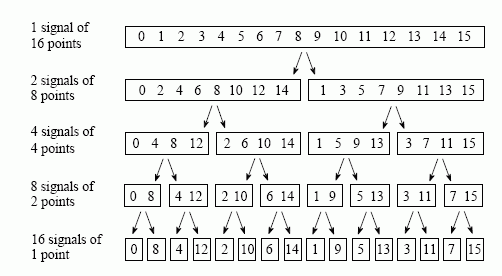
\includegraphics[width=1\textwidth,center]{resources/images/split.png}
			\end{figure}
		\end{column}
		\begin{column}{0.50\textwidth}
			\begin{figure}
				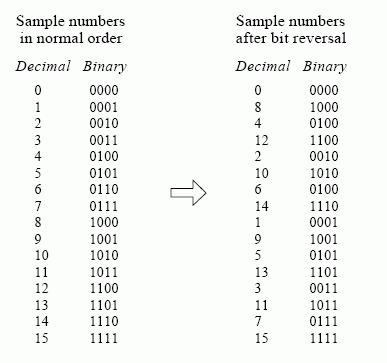
\includegraphics[width=1\textwidth,center]{resources/images/reverse.png}
			\end{figure}
		\end{column}
	\end{columns}

	\endgroup
\end{frame}

\begin{frame}
	\begingroup
	\small
	\begin{figure}
		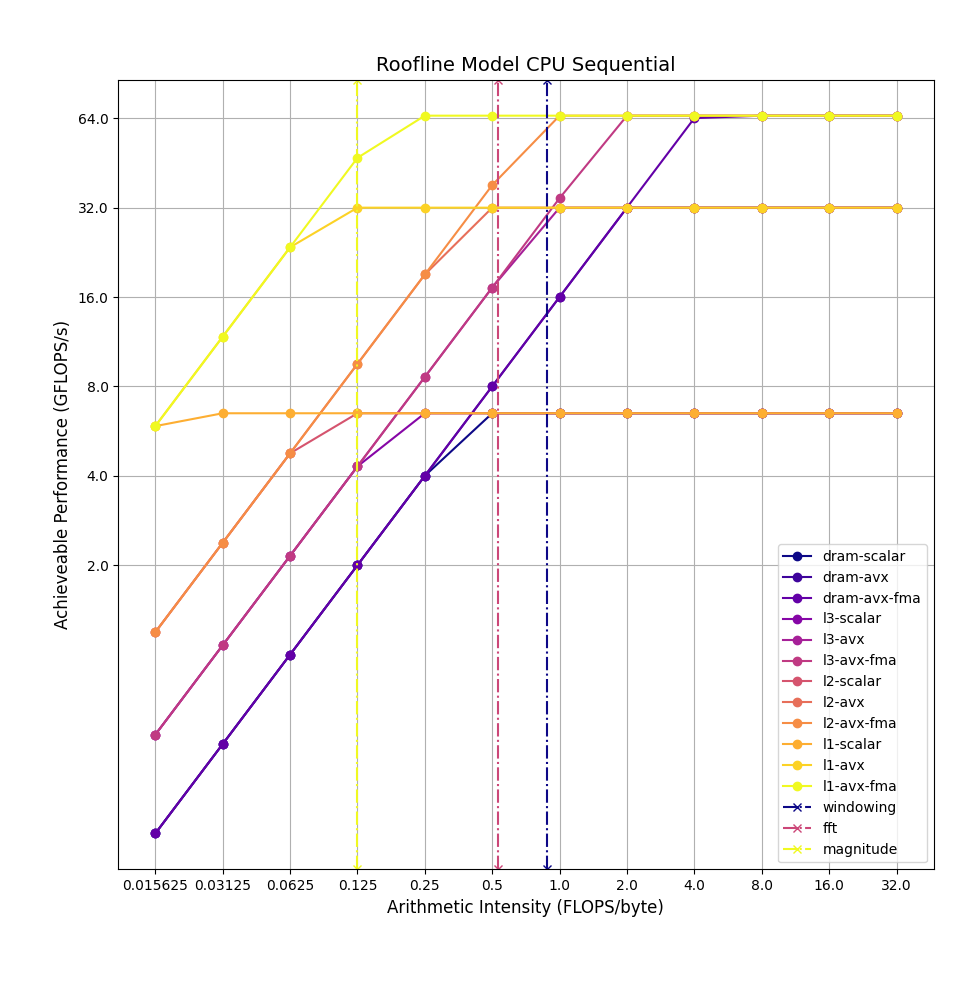
\includegraphics[width=0.75\textwidth,center]{resources/images/roof-seq-cpu.png}
	\end{figure}
	\endgroup
\end{frame}

\begin{frame}
	\begingroup
	\small
	\begin{figure}
		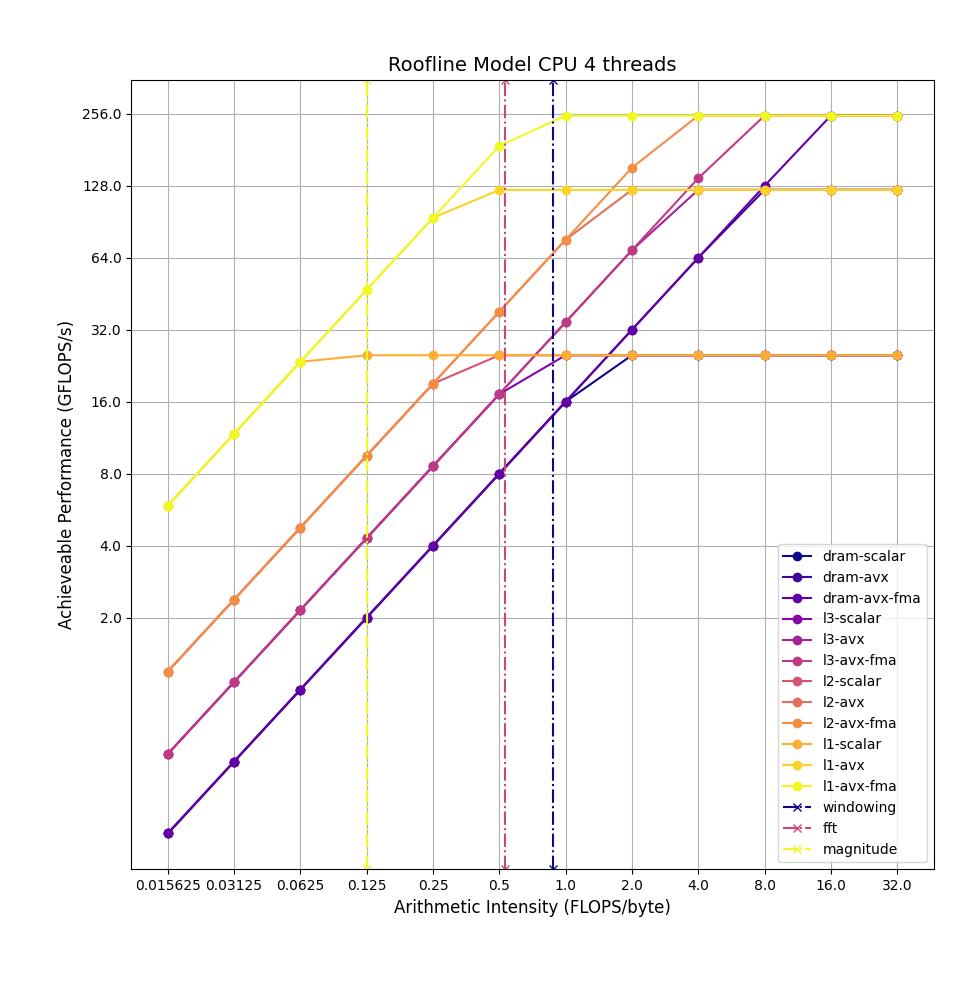
\includegraphics[width=0.75\textwidth,center]{resources/images/roof-mt4-cpu.png}
	\end{figure}
	\endgroup
\end{frame}

\begin{frame}
	\begingroup
	\small
	\begin{figure}
		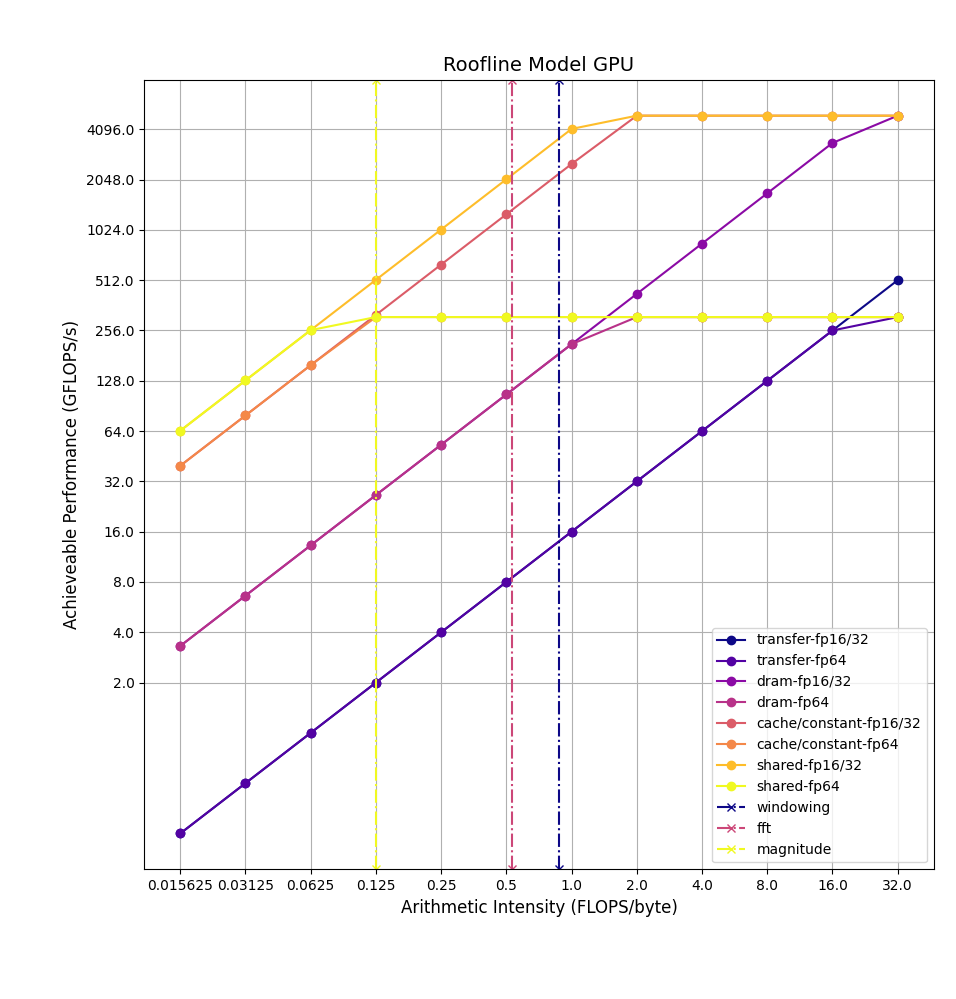
\includegraphics[width=0.75\textwidth,center]{resources/images/roof-gpu.png}
	\end{figure}
	\endgroup
\end{frame}

\begin{frame}{Correctness}
	\begingroup
	\small
	\begin{itemize}
		\item Use FFTW as reference as it scientifically proven to be extremely
		accurate (between $10^{-16}$ and $10^{-15}$ rms error on x86\_64).
		\item First four numbers of the mantissa must match...
		\item Except for first and last element they only require two numbers
		\item Require any exponent between $10^{-250}$ and $10^{250}$ must
		match exactly for all elements
	\end{itemize}
	\endgroup
\end{frame}

\begin{frame}{Upcoming challanges}
	\begingroup
	\small
	\begin{itemize}
		\item Porting algorithm to OpenCL, first priority
		\item Performing initial performance measurements
		\item Determining current bottleneck 
		\begin{itemize}
			\item Memory access patterns, windowing \& FFT strides?
			\item Special mathematical operations $cos$, $sin$, $sqrt$?
		\end{itemize}
	\end{itemize}
	\endgroup
\end{frame}

\end{document}